\documentclass{article}

% if you need to pass options to natbib, use, e.g.:
%     \PassOptionsToPackage{numbers, compress}{natbib}
% before loading neurips_2020

% ready for submission
% \usepackage{neurips_2020}

% to compile a preprint version, e.g., for submission to arXiv, add add the
% [preprint] option:
%     \usepackage[preprint]{neurips_2020}

% to compile a camera-ready version, add the [final] option, e.g.:
%     \usepackage[final]{neurips_2020}

% to avoid loading the natbib package, add option nonatbib:
\usepackage{neurips_2020}

\usepackage[utf8]{inputenc} % allow utf-8 input
\usepackage[T1]{fontenc}    % use 8-bit T1 fonts
\usepackage{hyperref}       % hyperlinks
\usepackage{url}            % simple URL typesetting
\usepackage{booktabs}       % professional-quality tables
\usepackage{amsfonts}       % blackboard math symbols
\usepackage{nicefrac}       % compact symbols for 1/2, etc.
\usepackage{xcolor}
\usepackage{ulem}

\usepackage{microtype}      % microtypography
\usepackage{amsmath}
\usepackage{graphicx}
\usepackage{arydshln}

\usepackage[lofdepth,lotdepth]{subfig}
\usepackage{pifont}
 
\newcommand{\Edouard}[1]{\textcolor{blue}{#1}}
\newcommand{\mynotes}[1]{\textcolor{red}{#1}}
\title{Random Patches in Image Classification}


% The \author macro works with any number of authors. There are two commands
% used to separate the names and addresses of multiple authors: \And and \AND.
%
% Using \And between authors leaves it to LaTeX to determine where to break the
% lines. Using \AND forces a line break at that point. So, if LaTeX puts 3 of 4
% authors names on the first line, and the last on the second line, try using
% \AND instead of \And before the third author name.

\author{%
  Louis Thiry \\
  Departement d'informatique \\
  ENS, PSL University, Paris\\
  \texttt{louis.thiry@ens.fr} \\
  \And
  Michael Arbel\\
  Gatsby\\
  Computational Neuroscience Unit\\
  University College London\\
  \texttt{michael.n.arbel@gmail.com}\\
  \And
    Eugene Belilovsky\\
  Mila, University of Montreal\\
  \texttt{eugene.belilovsky@umontreal.ca}
  \And
  Edouard Oyallon \\
  CNRS/LIP6 \\
  Sorbonne University \\
  \texttt{edouard.oyallon@lip6.fr} \\
}

\begin{document}
\appendix

\section{Mahanalobis distance and whitening}

The Mahalanobis distance \citep{chandra1936generalised, mclachlan1999mahalanobis} between two samples $x$ and $x'$ drawn from a random vector $X$ with covariance $\Sigma$ is defined as  
\begin{align*} D_M (x, x' ) =  \sqrt{ (x - x')^T \Sigma^{-1} (x - x')} \end{align*}
If the random vector $X$ has identity covariance, it is simply the usual euclidian distance : 
\begin{align*} D_M (x, x' ) =  \| x - x' \| \ .\end{align*}

Using the diagonalization of the coraviance matrix,  $\Sigma = P\Lambda P^T$, the affine whitening operators of the random vector $\mathbf{X}$ are the operators 
\begin{equation}
\label{whitening}
     w : \mathbf{X} \mapsto O \Lambda^{-1/2} P^T (\mathbf{X} - \mu), \quad \forall O \in  O_n (\mathbb{R}) \ .
\end{equation}
For example, the PCA whitening operator is 
\begin{equation*}
     w_{\rm PCA} : \mathbf{X} \mapsto \Lambda^{-1/2} P^T (\mathbf{X} - \mu)
\end{equation*}
and the ZCA whitening operator is 
\begin{equation*}
     w_{\rm ZCA} : \mathbf{X} \mapsto P \Lambda^{-1/2} P^T (\mathbf{X} - \mu) \ .
\end{equation*}
For all whitening operator $w$ we have
\begin{align*}
\|w(x) - w(x')\| = D_M(x, x')
\end{align*}
since
\begin{align*}
  \|w(x) - w(x')\|
    &= \| O \Lambda^{-1/2} P^T ( x - x') \|\\
    &= \sqrt{(x - x')^T P \Lambda^{-1/2} O^T O \Lambda^{-1/2} P^T (x - x') }\\
    &=  \sqrt{ (x - x')^T P \Lambda^{-1} P^T (x - x')} \\
    &= D_M(x, x') \ .
\end{align*}

\section{Implementation of the patches K-nearest-neighbors  encoding}

In this section, we explicitly write the whitened patches with the whitening operator $W$.
Recall that  we consider the following set of euclidean pairwise distances:
\begin{align*}\mathcal{C}_{i, x} =\{\Vert W p_{i, x} - W d \Vert\, d\in\mathcal{D} \}\,.\end{align*}

For each image patch we encode the $K$ nearest neighbors of $W p_{i,x}$ in the set $Wd, d \in \mathcal{D}$, for some $ K \in 1 \ldots|\mathcal{D}| $.
We can use the square distance instead of the distance since it doesn't change the $K$ nearest neighbors.
We have 
\begin{align*}
    \Vert Wp_{i,x} - Wd \Vert^2 = \Vert Wp_{i,x} \Vert^2 - 2 \langle p_{i,x}, W^T W d \rangle + \Vert Wd\|^2
\end{align*}
The term $\|Wp_{i,x}\|^2$ doesn't affect the $K$ nearest neighbors, so the $K$ nearest neighbors are the $K$ smallest values of
\begin{align*}
        \left \lbrace {\|Wd \|^2 \over 2} + \langle p_{i,x}, -W^T W d \rangle, \ d \in \mathcal{D} \right \rbrace
\end{align*}
This can be implemented in a convolution of the image using $-W^T W d$ as filters and $\|Wd \|^2 / 2$ as bias term, followed by a "vectorwise" non-linearity that binary encodes the $K$ smallest values in the channel dimension.
Once this is computed, we can then easily compute 
\begin{align*}
        \left \lbrace {\|Wd \|^2 \over 2} + \langle p_{i,x}, W^T W d \rangle, \ d \in \mathcal{D} \right \rbrace
\end{align*}
which is the quantity needed to compute the $K$ nearest neighbors in the set of negative patches $\overline{\mathcal{D}}$.
This is a computationally efficient way of doubling the number of patches while making the representation invariant to negative transform.


\section{Ablation study on CIFAR-10}

For this ablation study on CIFAR-10, the reference experiment uses  $|\mathcal{D}|=2048$ patches, a patch size $Q=6$ a number of neighbors $K=0.4\times 2048 = 820$ and a whitening regularizer $\lambda=1e-3$, and yields 82.5\% accuracy.
Figure \ref{fig:ablation_study_highres} shows the results in high resolution.

\begin{figure}[h!]
  \centering
   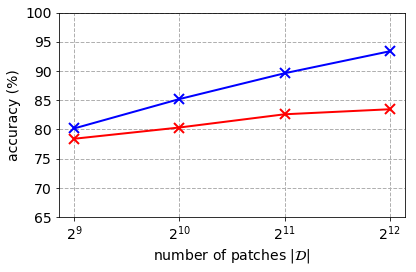
\includegraphics[width=0.49\linewidth]{figures/ablation_npatches_large.png}
  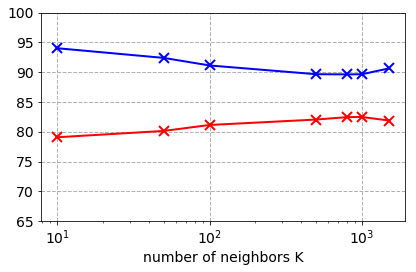
\includegraphics[width=0.49\linewidth]{figures/ablation_K_large.png}
  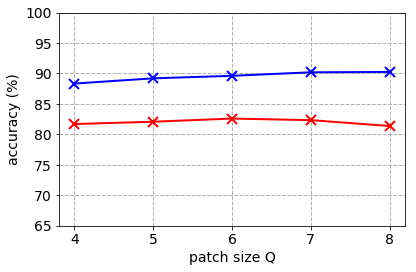
\includegraphics[width=0.49\linewidth]{figures/ablation_Q_large.png}
  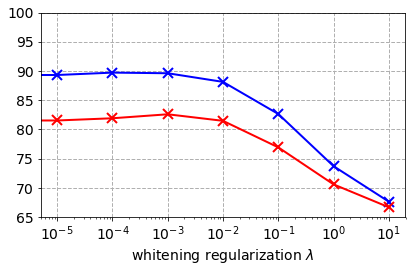
\includegraphics[width=0.49\linewidth]{figures/ablation_lambda_large.png}\\
    \caption{CIFAR-10 ablation experiments, train accuracies in blue, test accuracies in red.
    Number of patches $|\mathcal{D}|$ varies in $\lbrace 512, 1024, 2048, 4096  \rbrace$, number of neighbors $K$ varies in $\lbrace 10, 50, 100, 500, 800, 1000, 1500\rbrace$, patch size $Q$ varies in $\lbrace 4,5,6,7,8 \rbrace$, whitening regularization $\lambda$ varies in $\lbrace0, 10^{-5}, 10^{-4}, 10^{-3}, 10^{-2}, 10^{-1}, 1, 10 \rbrace$. }
    \label{fig:ablation_study_highres}
\end{figure}


\section{Intrinsic dimension estimate}

The following estimate of the intrinsic dimension $d_{\rm int}$ is introduced in \cite{Levina:2004} as follows
\begin{align}
	d_{\rm int}(p) = \left( \frac{1}{K-1} \sum_{k=1}^{K-1}\log \frac{\tau_K(p)}{\tau_k(p)} \right)^{-1} \, ,
\end{align}
where $\tau_k(p)$ is the euclidean distance between the patch $p$ and it's $k$-th nearest neighbor int  the training set.
\end{document}